%%%%%%%%%%%%%%%%%%%%%% Props %%%%%%%%%%%%%%%%%%%%%%
\documentclass{article}

\usepackage[french]{babel}
\usepackage[utf8]{inputenc}
\usepackage[T1]{fontenc}
\usepackage{graphicx}
\usepackage{fancyhdr}
\usepackage{eurosym}
\usepackage{color}
\usepackage{soul}
\usepackage{listings}
\usepackage{enumitem}
\usepackage{enumerate}
\usepackage{float}

\pagestyle{fancy}
\lhead{Manuel d'utilisation}
\chead{Deadly Science}
\rhead{Custos Carceris}

\title{Manuel d'utilisation}

\begin{document}

\maketitle
\tableofcontents

\newpage
\section{Menus}
\subsection{Menu Principal}

\begin{figure}[H]
	\centering
	
\includegraphics[width=0.49\textwidth]{MainMenu.png}
	\caption{Menu Principal}
	\label{Menu Principal}
\end{figure}

Lorsque vous lancez le jeu, vous arriverez sur l'écran principal où vous pourrez quitter le jeu, changer les paramètres ou encore entrer dans une salle.
\paragraph{Paramètres}

Dans ce menu, vous pouvez changer la configuration des touches en cliquant sur le bouton de l'action dont vous souhaitez modifier la touche d'exécution, puis en pressant la touche que vous souhaitez y affecter. Elle devrait alors s'afficher sur le bouton à la place de l'ancienne : la modification vient d'être effectuée. Vous pouvez également changer de langue en appuyant sur le bouton "Langue", puis en choisissant celle qui vous sied le mieux. Vous pouvez aussi changer votre pseudonyme en écrivant le nom que vous souhaitez dans la barre correspondante, et dans le cas où vous n'auriez pas d'idées, vous pouvez cliquer sur le bouton "Aléatoire" pour en générer directement un qui sera, comme le bouton l'indique, aléatoire. A l'aide des jauges sur la droite, vous pouvez en outre modifier le volume des sons et musiques, ainsi que le degré de sensibilité de la souris dans le jeu.

\begin{figure}[H]
	\centering
	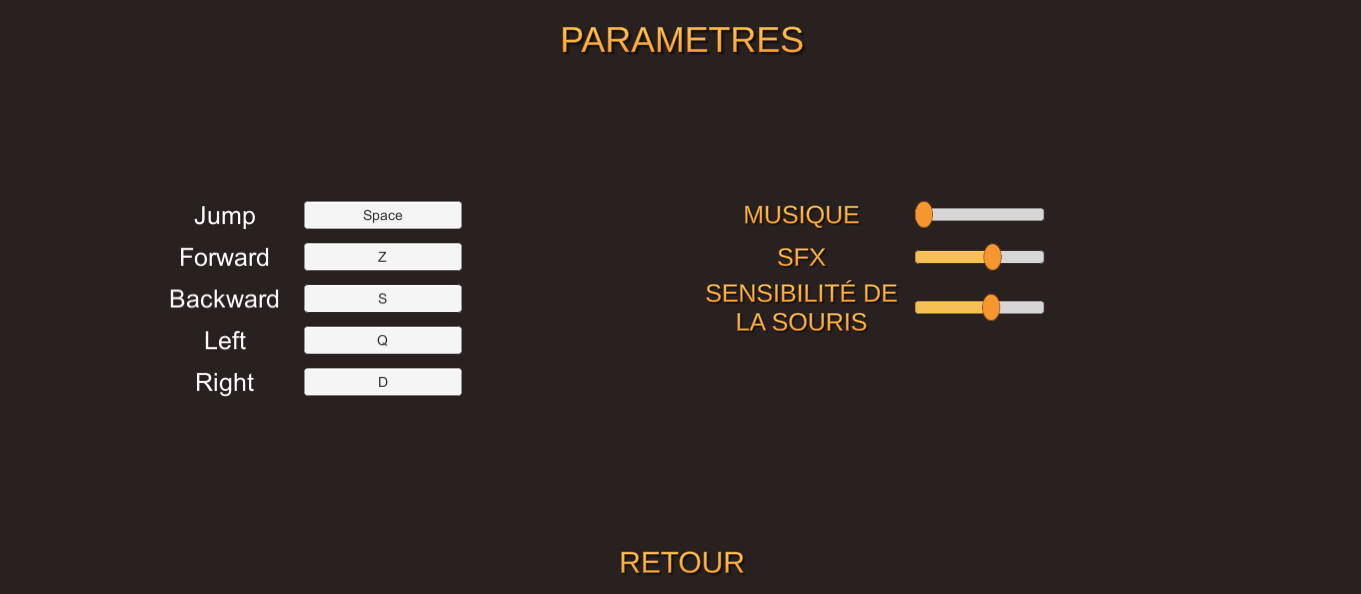
\includegraphics[width=0.49\textwidth]{parametres.png}
	\caption{Paramètres}
	\label{Paramètres}
\end{figure}


\paragraph{}
Une fois que vos paramètres sont configurés comme vous le souhaitez, vous pouvez cliquer sur "Jouer".

\subsection{Enter dans une salle}
Pour entrer dans une salle, il existe deux méthodes ; soit vous en créez une, soit vous rejoignez une salle déjà existante.

\paragraph{Créer une salle}
Pour créer une salle standard, il suffit de cliquer sur la barre de texte, écrire le nom de la salle que vous souhaitez puis cliquer sur "Créer une salle".

\begin{figure}[H]
	\centering
	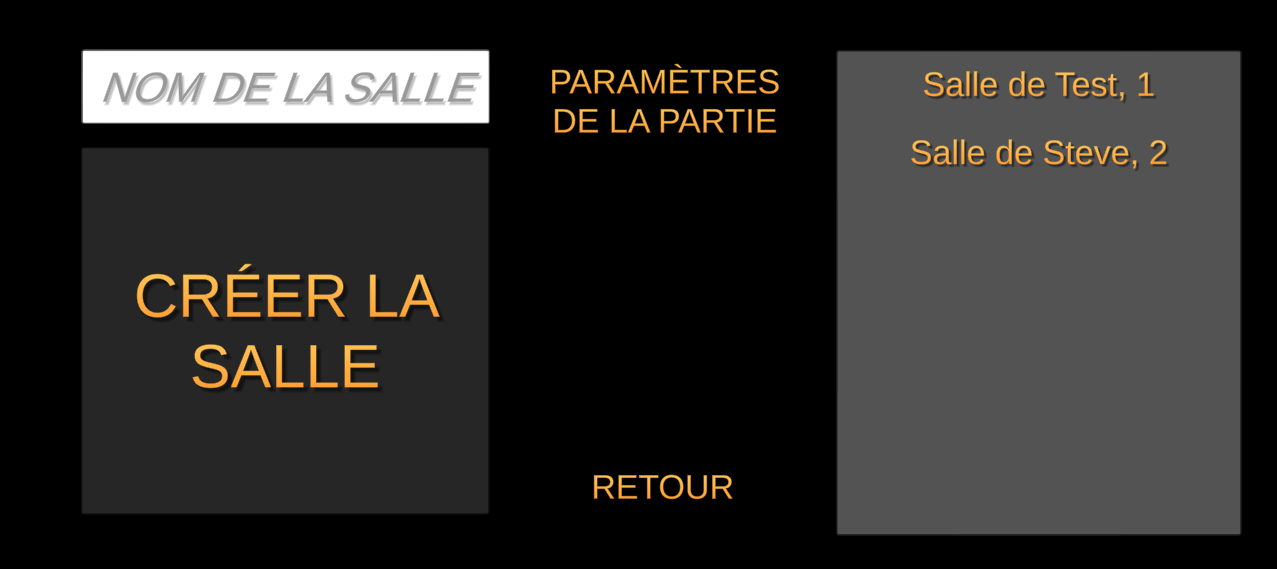
\includegraphics[width=0.49\textwidth]{Menu1.png}
	\caption{Menu pour créer une salle}
	\label{Menu pour créer une salle}
\end{figure}

Cependant, la salle par défaut lancera une partie pour quatre joueurs, en mode Classique, dans un labyrinthe de dimensions 10x10.
Si vous souhaitez modifier au moins l'un de ces paramètres, vous pouvez aisément les changer en cliquant sur Paramètres de la partie, et vous serez alors emmené dans un autre menu.

\begin{figure}[H]
	\centering
	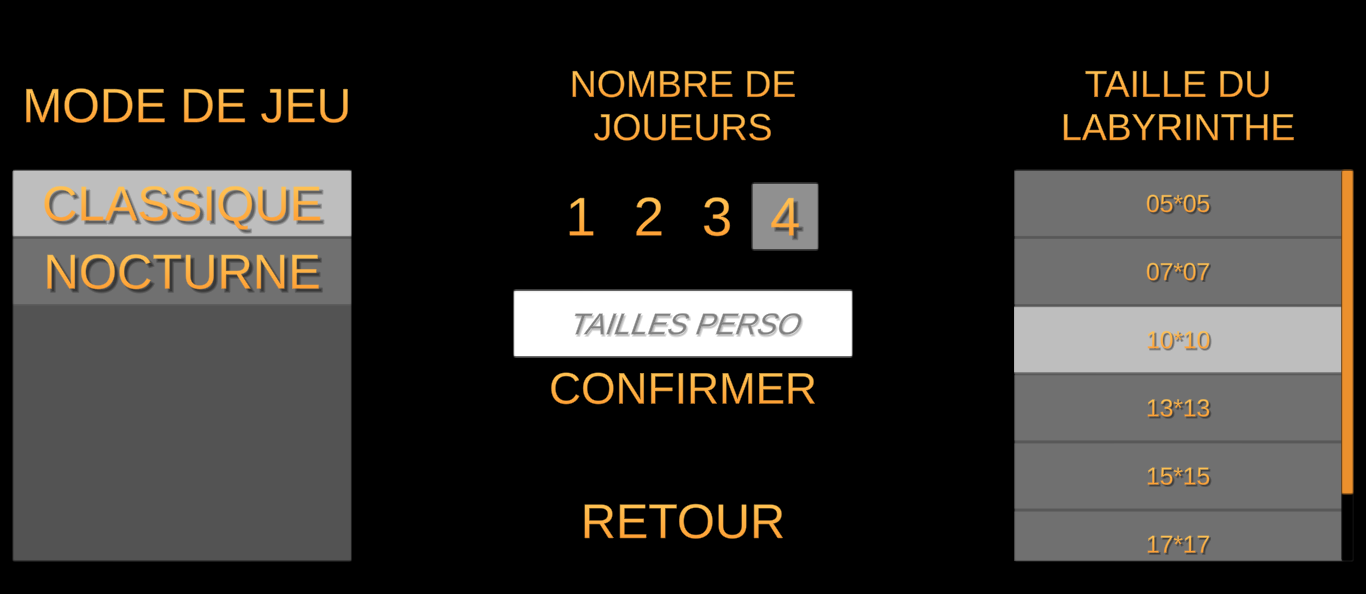
\includegraphics[width=0.49\textwidth]{Menu2.png}
	\caption{Menu pour paramétrer une salle}
	\label{Menu pour paramétrer une salle}
\end{figure}

\paragraph{Configurer une salle}
Dans ce menu, vous pouvez modifier le nombre de joueurs attendus dans la salle, le mode de jeu de la partie, et enfin les dimensions du labyrinthe. Pour changer le nombre de joueurs dans le labyrinthe, il suffit de cliquer sur le nombre de joueurs que vous souhaitez. Attention, cependant, il faut que vous gardiez en tête que le nombre de joueurs influence le déroulement de la partie. Pour changer le mode de jeu, il s'agit de la même procédure, cliquez simplement sur celui que vous souhaitez dans la colonne de gauche. Les paramètres choisis ont un fond blanc. 

\paragraph{Changer la taille du labyrinthe}
Pour changer la taille du labyrinthe, vous pouvez soit cliquer sur l'une des tailles prédéfinies dans la colonne de droite, soit écrire une taille personnalisée dans la barre blanche puis en appuyant sur "Confirmer". Assurez vous de respecter le format "00*00", en remplaçant les 0 par les valeurs que vous souhaitez affecter aux dimensions du dédale. Si tel n'est pas le cas, votre configuration ne sera pas prise en compte. De même, si votre configuration nécessite trop de salles ou, au contraire, trop peu, elle ne sera pas non plus prise en compte. Pour information, un labyrinthe doit toujours avoir au moins 8 salles, et toujours au plus 400 cases. Si, en revanche, vous préférez sélectionner une dimension prédéfinie, vous n'aurez qu'à cliquer sur le bouton correspondant. Notez bien que pour accéder aux dimensions les plus importantes, vous pouvez utiliser la molette pour faire coulisser le contenu de la colonne de droite. Une fois que vous aurez fini de configurer les paramètres de votre future partie, appuyez simplement sur "Retour", et créez une salle.

\paragraph{}
Pour rejoindre une partie, il suffit d'être dans le menu précédent et de cliquer sur la salle que vous souhaitez rejoindre dans la colonne à droite de l'écran. Vous verrez le nom des salles disponibles ainsi que le nombre de joueurs présents. Si la salle est complète, elle ne sera pas visible. 

\paragraph{A l'intérieur de la salle}
A droite de l'écran, vous pouvez voir la liste des joueurs présents dans la partie. Si vous êtes le Créateur de la salle, vous ne pourrez commencer la partie que si le nombre de joueurs correspond à celui de la salle, et que tous les joueurs présents dans la salle sont prêts, excepté vous, bien sûr. Vous pouvez voir si les autres joueurs sont prêts par les mentions "Prêt" et "Non Prêt" à côté de leur pseudonyme, à droite de l'écran.

\begin{figure}[H]
	\centering
	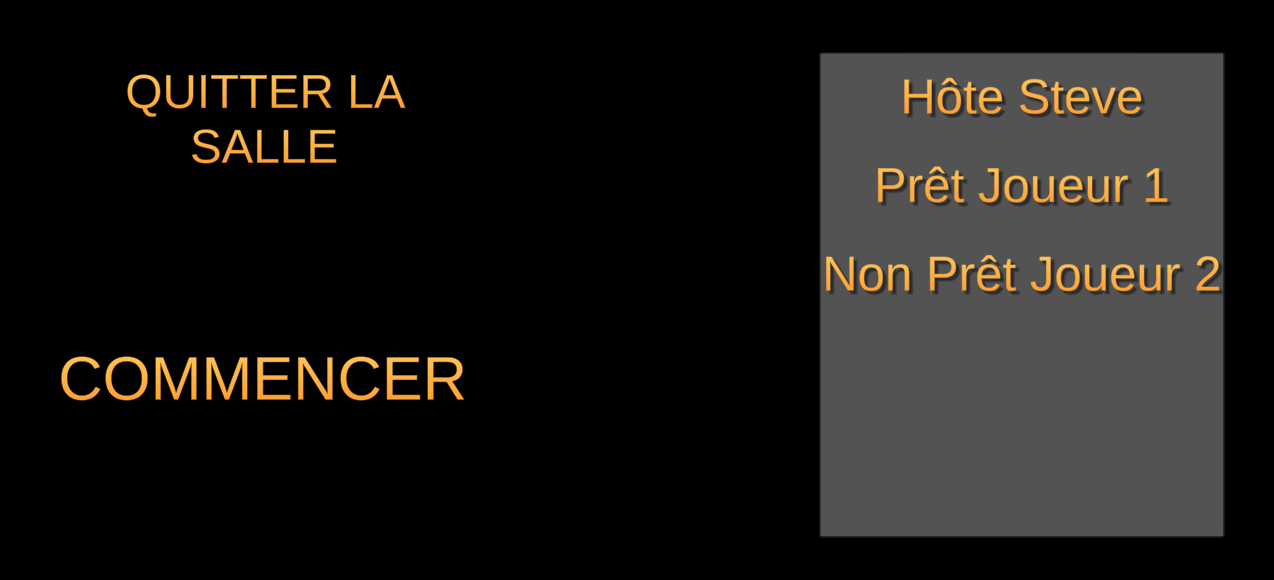
\includegraphics[width=0.49\textwidth]{Menu31.png}
	\caption{Menu lorsque l'on est l'hôte}
	\label{Menu lorsque l'on est l'hôte}
\end{figure}

Si, en revanche, vous avez rejoint la salle déjà créée, vous pouvez modifier votre "disponibilité" en cliquant sur le bouton "Prêt". Le bouton changera en fonction de votre "disponibilité" actuelle, ce que vous permet d'indiquer que vous n'êtes tout compte fait pas prêt à jouer, pour n'importe quelles raisons. Vous pouvez aussi voir votre "disponibilité" sur la liste des joueurs à droite de l'écran, tout comme le Créateur de la salle. 

\begin{figure}[H]
	\centering
	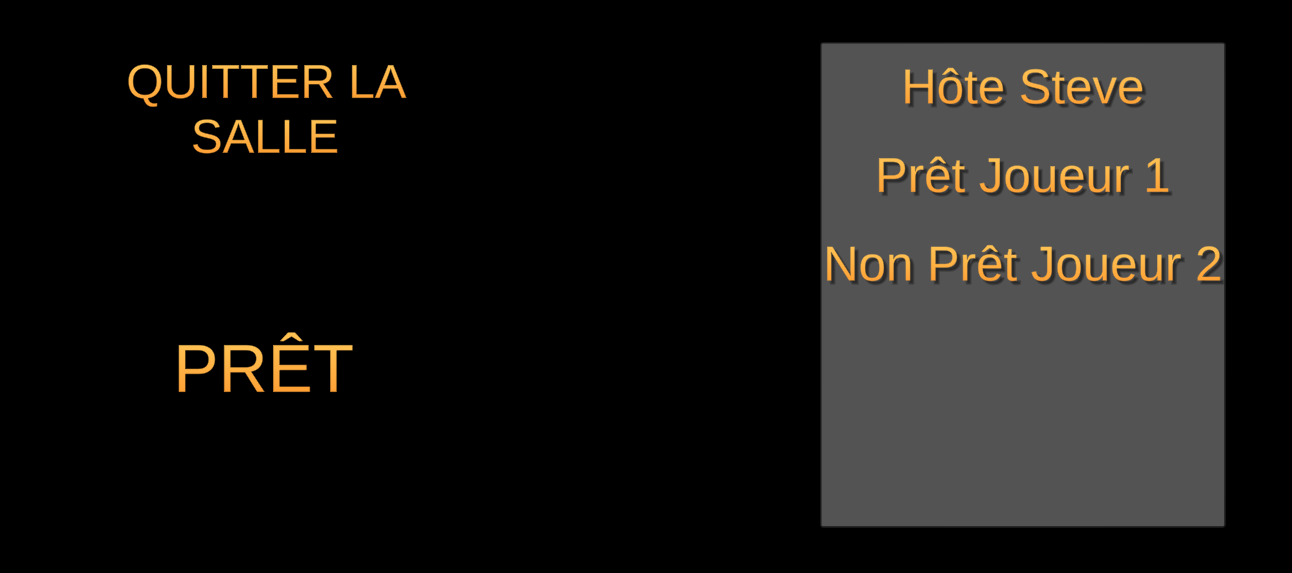
\includegraphics[width=0.49\textwidth]{Menu32.png}
	\caption{Menu lorsque l'on n'est pas l'hôte}
	\label{Menu lorsque l'on n'est pas l'hôte}
\end{figure}

\newpage
\section{Jeu}
\subsection{Première phase}

Une fois que vous êtes en jeu, vous commencez en tant qu'Infecté, et votre objectif est alors de chercher un sérum.

\begin{figure}[H]
	\centering
	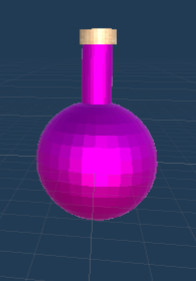
\includegraphics[width=0.49\textwidth]{Fioles.png}
	\caption{Sérum}
	\label{Sérum}
\end{figure}

Votre objectif actuel est affiché en haut à droite de l'écran, votre pseudonyme en haut à gauche de l'écran, et les objets qui sont actifs sur vous en bas à droite de l'écran. Vous pouvez savoir votre état en fonction de la couleur de votre pseudonyme : en magenta, vous êtes infecté, en vert, vous êtes guéri, en rouge, il est trop tard pour que vous puissiez être guéri, et en gris, vous êtes guéri, et personne ne peut vous voir ni vous réinfecter.

\begin{figure}[H]
	\centering
	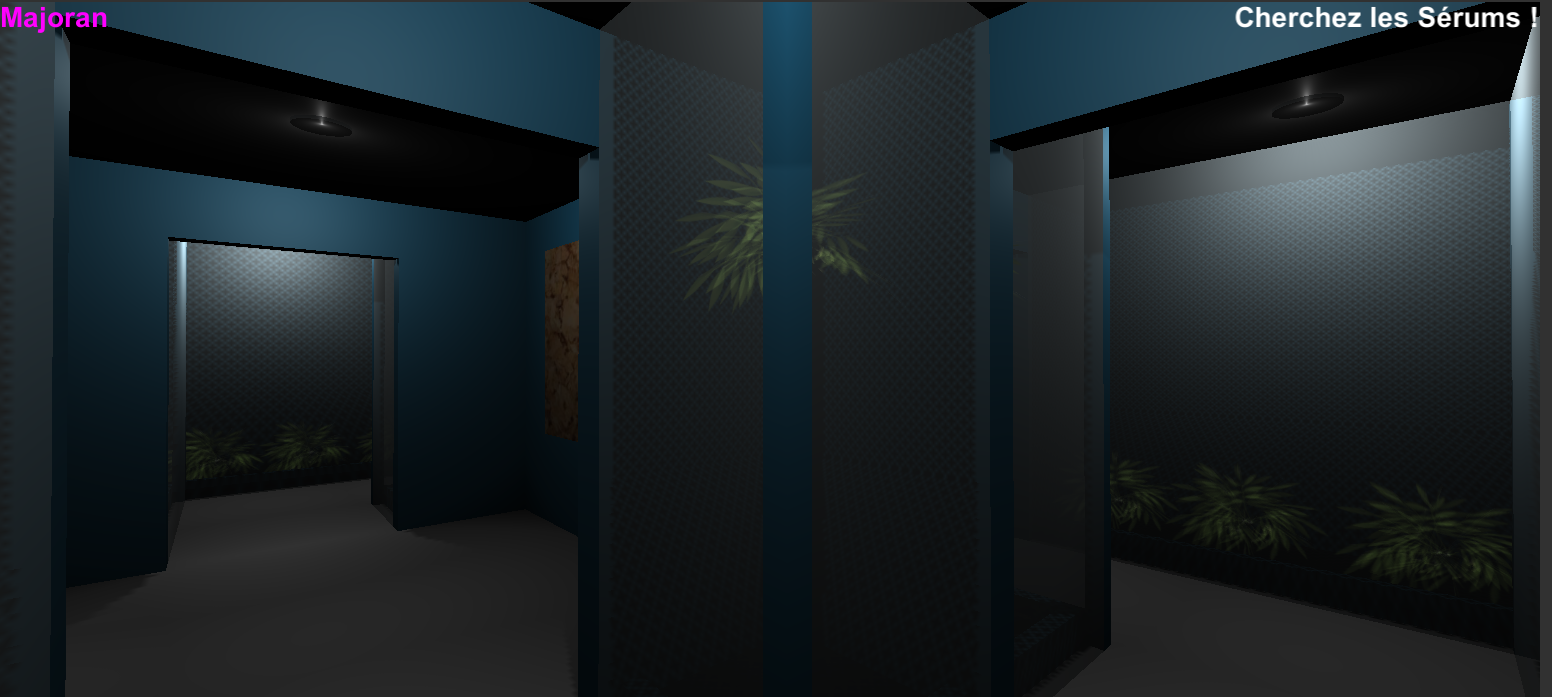
\includegraphics[width=0.49\textwidth]{Lumieres.png}
	\caption{A l'intérieur de la partie}
	\label{A l'intérieur de la partie}
\end{figure}

A l'aide des touches configurées dans les paramètres, vous pouvez vous déplacer dans le labyrinthe. Si vous voulez les changer en pleine partie, il vous suffit d'appuyer sur la touche "Echap", et de les reconfigurer à nouveau. A noter que vu que le jeu est synchronisé en réseau, les autres joueurs continuent à jouer pendant que vous êtes dans ce menu. Lorsqu'un joueur est à proximité et en face de vous, vous pouvez lui envoyer un coup de poing en faisant un clic gauche. Ceci lui fera baisser sa barre d'endurance. Lorsque sa jauge tombe à zéro, le joueur que vous venez de molester sera sonné : il sera ralenti et ne pourra plus se battre pendant un certain temps.

\subsection{Deuxième phase}

Lorsque tous les joueurs sauf un (excepté bien sûr si vous jouez seul) sont guéris, les joueurs guéris doivent échapper au joueur condamné, et joueur condamné, par esprit de vengeance, doit les recontaminer. Pour cela, le corrompu peut soit les toucher, soit les frapper. Lorsque le minuteur affiché en haut à gauche de l'écran arrive à zéro et que certains joueurs sont encore sains, ce sont ces joueurs guéris qui gagnent. En revanche, si tous les joueurs guéris ont été réinfectés avant la fin du décompte, c'est le premier joueur à avoir été condamné, autrement dit celui qui n'a pas eu l'occasion de récupérer un sérum, qui remporte la victoire. Quand un joueur se fait recontaminer, il doit aider les autres joueurs condamnés à recontaminer les joueurs guéris restants, mais quoiqu'il arrive, sa partie s'achèvera par une défaite.

Pour aider les joueurs, il existe multiples objets qui sont affichés comme montré sur la Figure 9 pour vous aider ou vous ralentir dans cette course contre la montre. La liste des objets, ainsi que leurs effets, sont indiqués sur notre site Web dans la partie Codex Plaga.

\begin{figure}[H]
	\centering
	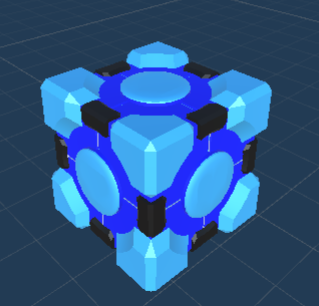
\includegraphics[width=0.49\textwidth]{Objet.png}
	\caption{Objet}
	\label{Objet}
\end{figure}

Lorsque vous arrivez à l'écran de fin, qui correspond soit à une victoire, soit à une défaite, vous pouvez cliquer sur "Quitter" pour quitter le jeu. Pour recommencer une autre partie, il suffit de relancer le jeu.

Sur ce, il ne nous reste plus qu'à vous souhaiter bonne chance, si vous souhaitez survivre aux laboratoires de Deadly Science ; vous en aurez besoin...
\end{document}
